\section{Proposed Approach} \label{sec:approach}
 
\subsection{Dataset and Preprocessing} \label{sec:dataset}

The dataset we will be utilizing is the UTKFace dataset \cite{app1},
which consists of $23,708$ aligned and cropped facial RGB images, 
annotated with age, gender, and ethnicity labels.
This dataset was created with the intention of covering
a wide range of variations, including pose, facial expression,
illumination, occlusion, resolution, and more.
In our analysis, we will specifically concentrate
on the first two attributes within the dataset: age and gender. 

In our analysis, we will exclusively consider $70\%$
of the dataset for our training set, with the remaining
$30\%$ designated for testing purposes.
This division allows us to train our models on a substantial
portion of the data while maintaining a separate,
untouched set for rigorous evaluation.

The training set exhibits an age distribution depicted
in the histogram
shown in Fig.~\ref{1age}, along with a balanced gender distribution,
as illustrated in Fig.~\ref{2gender1}.

\begin{figure}[htbp]
    \centerline{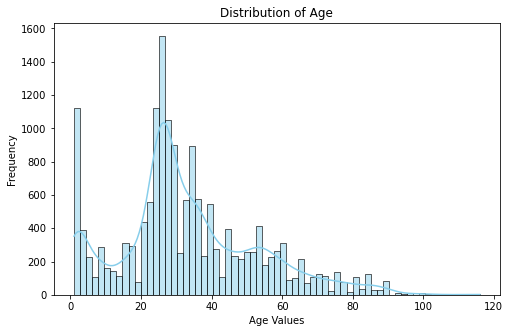
\includegraphics[width=.5\textwidth]{images/dataset/age.png}}
    \caption{Histogram of age distribution in the training set}
    \label{1age}
\end{figure}

\begin{figure}[htbp]
    \centerline{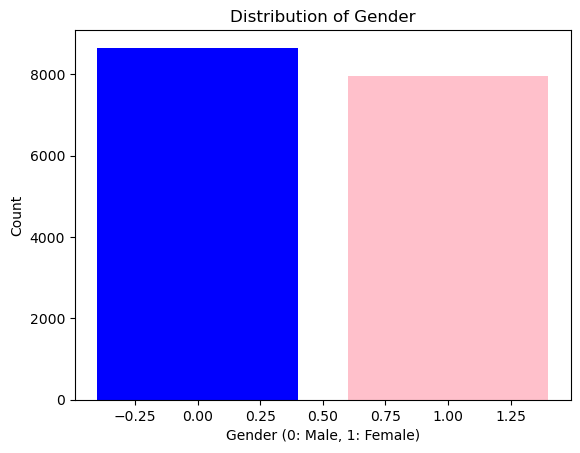
\includegraphics[width=.4\textwidth]{images/dataset/gender1.png}}
    \caption{Histogram of gender distribution in the training set}
    \label{2gender1}
\end{figure}

We further split the training set into a $70\%$ training set and a $30\%$
validation set. The validation set plays a critical role in refining
and making our model more robust, preventing overfitting through techniques
such as early stopping.

Despite this subdivision, we have taken measures to maintain the
balance in the dataset: the accompanying histogram  in Fig.~\ref{3gender2}
illustrates that, concerning gender,
the distribution remains similar in both datasets.

\begin{figure}[htbp]
    \centerline{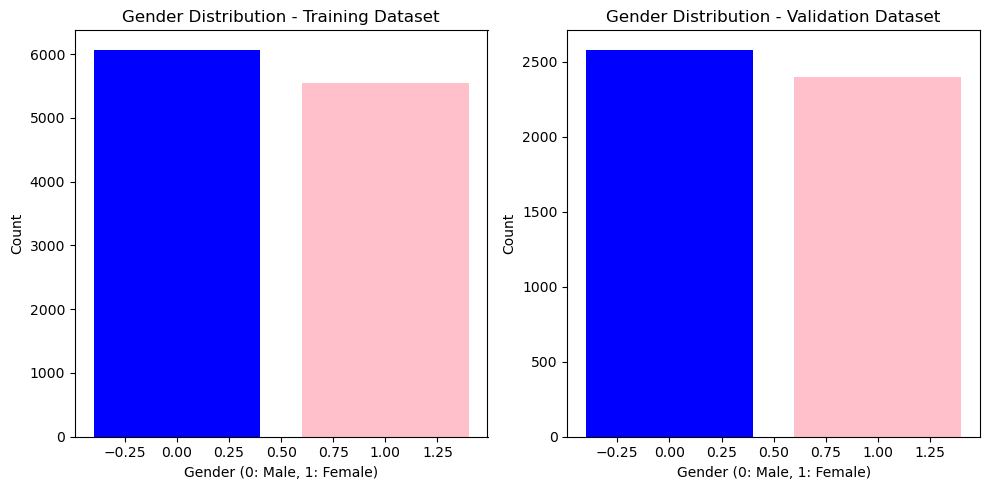
\includegraphics[width=.5\textwidth]{images/dataset/gender2.png}}
    \caption{Histogram of gender distribution in the new training
    set and the validation set}
    \label{3gender2}
\end{figure}

As for age, a continuous value that poses challenges for balance
assessment, we will employ the non-parametric Kolmogorov-Smirnov test
to scrutinize the absence of statistically significant differences in
the distributions of its values between the two datasets
(its null hypothesis) \cite{app2}.
The outcome of the aforementioned test yields a $p$-value of approximately
$0.38$, this value is reasonably high,
leading us to consider it sufficient evidence to accept the null hypothesis.
Thus, we conclude that the two distributions of age in the two
datasets do not exhibit statistically significant differences.
In the plot shown in Fig.~\ref{4CDFage}, we can observe that
the cumulative distribution functions of the age values of the
two datasets are almost identical.

\begin{figure}[htbp]
    \centerline{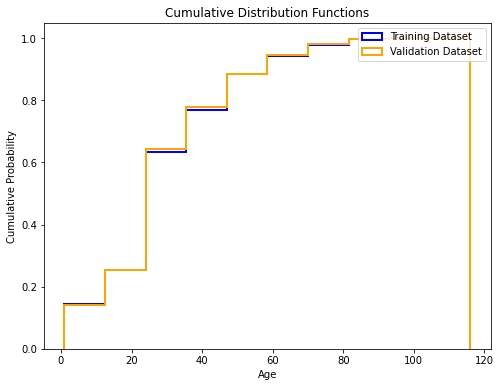
\includegraphics[width=.5\textwidth]{images/dataset/CDF_age.png}}
    \caption{CDF of age values in the
    new training set and the validation set}
    \label{4CDFage}
\end{figure}

The concluding step in our dataset preprocessing involves the application
of data augmentation techniques. Specifically, we expand the dataset
by incorporating horizontally mirrored images and introducing random
rotations of up to 10 degrees. Additionally, we employ random adjustments
to the brightness, contrast, saturation, and hue of the images.
This augmentation strategy has been employed based on empirical
evidence suggesting that enlarging the dataset enhances the performance
of the model \cite{app4}. By introducing these variations in orientation and color,
we aim to expose the model to a more diverse set of examples,
ultimately improving its ability to generalize and make accurate
predictions on unseen data.

\subsection{Model Architecture} \label{sec:model}

As previously mentioned, in this project, we will compare two
CNN architectures, one comprising a single multi-task
network and another consisting of two single-task networks.
The overarching goal is common between them.

Let's delve into the details of the both architectures.

\subsubsection{Multi-task Architecture} \label{sec:multi}

The multi-task architecture, shown in Fig.~\ref{cnn1},
features a structure of the following type:
$$ \text{\texttt{INPUT}} \rightarrow [\text{\texttt{CONV}} \rightarrow \text{\texttt{BATCHNORM}} \rightarrow \text{\texttt{RELU}} \rightarrow \text{\texttt{MAXPOOL}}] \rightarrow $$
$$\rightarrow [\text{\texttt{CONV}} \rightarrow \text{\texttt{RELU}} \rightarrow \text{\texttt{MAXPOOL}}]\times 3$$
it then divides it into two branches, each retaining the same structure:
$$ \text{\texttt{FC}} \rightarrow \text{\texttt{DROPOUT}} \rightarrow \text{\texttt{RELU}} \rightarrow \text{\texttt{FC}}$$
The key distinction lies in the purpose of each branch:
one branch is designed to address the classification problem,
specifically predicting gender,
so it has two output neurons that perform a softmax function.
\begin{figure}[htbp]
    \centerline{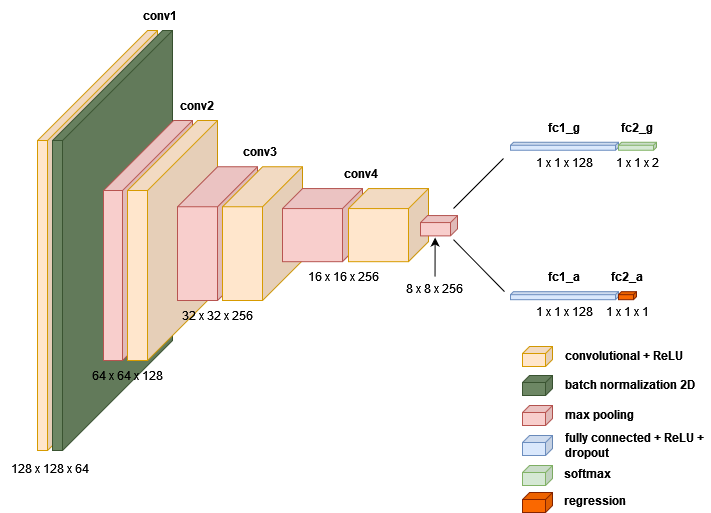
\includegraphics[width=.5\textwidth]{images/shared_cnn.png}}
    \caption{Graphical representation of the Multi-task architecture}
    \label{cnn1}
\end{figure}
The other branch is designed to solve the regression problem,
involving the prediction of age,
it has a single output neuron that performs a linear function.

Let's explore in more detail the structure of the various layers:
\begin{itemize}
    \item The input, with dimensions $128\times128\times3$, enters
    the first $2$D convolutional layer comprising $64$ filters of size $3\times3$.
    These filters apply a padding of $2$ to preserve spatial dimensions
    after convolution. The stride is set to $1$
    in the convolutional layer and set to $2$ in the subsequent 
    pooling layer. This setting avoids requiring the network to learn
    to subsample and it's repeated in all the subsequent layers.
    \item Following this, a batch normalization layer is applied
    to the output of the previous convolutional layer.
    Batch normalization helps stabilize and accelerate
    the training of neural networks by normalizing the batch to its
    mean and standard deviation instead of doing it with the whole dataset.
    This is the only occurrence of batch normalization in the network.
    \item The output of the batch normalization then enters
    the Rectified Linear Unit (RELU) activation function,
    it introduces non-linearity to the model,
    allowing it to learn from more complex patterns in the data.
    \item Before entering another convolutional layer,
    the output of the preceding layer undergoes pooling through
    a max pooling layer with a window size of $2\times2$ and a stride of 2.
    As a result, the size of the produced map is halved.
    \item The previous steps are repeated three more times,
    with the only difference being the number of filters in the
    second convolutional layer (5 instead of 3), the number of filters,
    which is doubled in each subsequent convolutional layer,
    and the absence of batch normalization layers.
    \item The output of the last pooling layer is flattened
    and fed into two spearated branches of fully connected layers,
    each with $128$ neurons,
    followed by a dropout layer (set at $0.25$) and ReLU activation.
    \item The output of the last fully connected layer of the first branch
    is fed into a fully connected layer with two neurons,
    one for each class of the classification problem
    (\texttt{Male} or \texttt{Female}), followed by a softmax activation.
    \item The output of the last fully connected layer of the second branch
    is fed into a fully connected layer with one neuron
    for the regression problem (age), followed by a linear activation.
\end{itemize}

Since we have incorporated a batch normalization layer,
it has proven unnecessary to include dropout layers in the convolutional part
of the network.
The combined use of these techniques is generally discouraged,
as a rule of thumb, since it tends to yield worse results than
when only one of them is employed \cite{app3}.
However, we have included a dropout layer in the fully connected part.

We utilize Cross Entropy Loss as the loss function for classification
and Mean Squared Error (MSE) Loss for regression.
These losses are summed and employed for backpropagation at each step.

We have employed an Adam optimizer with a learning rate set to $0.01$.

\subsubsection{Single-task Architecture} \label{sec:single}

The single-task architecture, shown in Fig.~\ref{cnn2},
features the same structure as the multi-task architecture,
with the only difference being that, instead of branching out
in two different layers for the tasks, it has a single branch
that performs either classification or regression.
For this reason, the single-task architecture is composed of
two separate networks, one for each task.

The loss functions used are the same as the ones employed
in the multi-task architecture, the only difference being
that, instead of summing them and using the sum for backpropagation,
we use them separately for each network.

We have employed an Adam optimizer with a learning rate set to $0.001$
for both the classification and the regression network.\\

\begin{figure}[htbp]
    \centerline{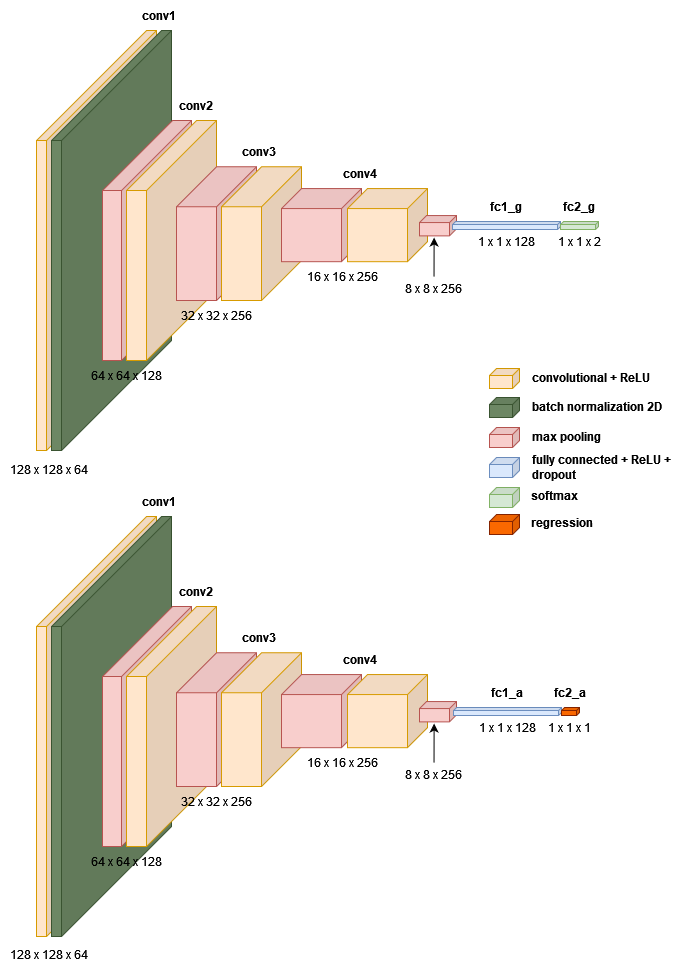
\includegraphics[width=.5\textwidth]{images/single_cnn.png}}
    \caption{Graphical representation of the Single-task architecture}
    \label{cnn2}
\end{figure}

In both architectures, the batch size is $64$.
The metrics used for evaluation are accuracy, defined as the ratio
of correctly predicted instances to the total instances, expressed as:

\[
\text{{Accuracy}} = \frac{\text{{Number of Correct Predictions}}}{\text{{Total Number of Predictions}}}
\]
for classification tasks, and R-squared ($R^2$) score, defined as the proportion of the variance in the dependent variable that is predictable from the independent variable(s), expressed as:

\[
R^2 = 1 - \frac{\sum_{i=1}^{n} (y_i - \hat{y}_i)^2}{\sum_{i=1}^{n} (y_i - \bar{y})^2}
\]
for regression tasks.